\section{Design Goal}\label{sec:goals}
The goal of the isolated driver domains is to provide strong isolation between a device driver and a monolithic kernel and at the same time to avoid modifications to the device driver code. The goal of the thesis is to reduce the performance penalty due to the communication between the domains. 

\subsection*{Performance Improvement}
The IDDR system is a re-implementation of isolated driver domains proposed by Fraser et. al. Even though IDDR system provides better robustness for the operating system, it suffers from performance overheads. The main reasons for the lower performance are the data copying overhead and the inter-domain communication overhead. 

\paragraph{Copying Overhead: } For write operation, a Linux system copies data from user space to kernel space and then from kernel space to the physical device. However, isolated driver domains system copies data from guest OS user space to guest OS kernel space, it then copies it to shared memory segment and from shared memory segment to the physical device. The extra copying of data in to the shared memory segment lowers the performance of the system. 

\paragraph{Communication Channel Overhead: } The application domain and the driver domain sends virtual interrupts when requests and responses are shared between both the domains. These virtual interrupts cause rescheduling of a domain in order to deliver the interrupts. Rescheduling of a domain can cause a context switch at an hypervisor level which adds an overhead to the system performance. Our goal is to reduce the overhead during communication between the driver domain and the application domain.

\section{Isolated Device Driver Properties}
\label{sec:properties}
This section covers the properties of the isolated driver domains. As we explore the opportunities to improve the performance of the isolated driver domains, it is necessary that these properties are not compromised.

\subsection*{Strong Isolation}
One of the main properties of the IDDR system is strong isolation. The isolated driver domains adds an extra layer of isolation in the design which provides fault isolation between the kernel and the device driver. It ensures that a bug within a device driver does not affect other kernel components.

\subsection*{Compatibility and Transparency} 
The extension of existing OS structures usually results in a large number of broken applications. Usually such extensions change the APIs visible to applications and breaks compatibility with the existing applications. The isolated driver domains does not change APIs visible to applications and device driver code and hence existing device drivers and applications are compatible with the new architecture.

\section{System Overview}\label{overview}

Figure~\ref{fig:monolithic} presents the architectural overview of the modern operating system with a monolithic kernel and Figure~\ref{fig:base IDDR system overview} presents the architectural overview of the IDDR system.
\\[3mm]
\begin{figure}[!ht]
\centering
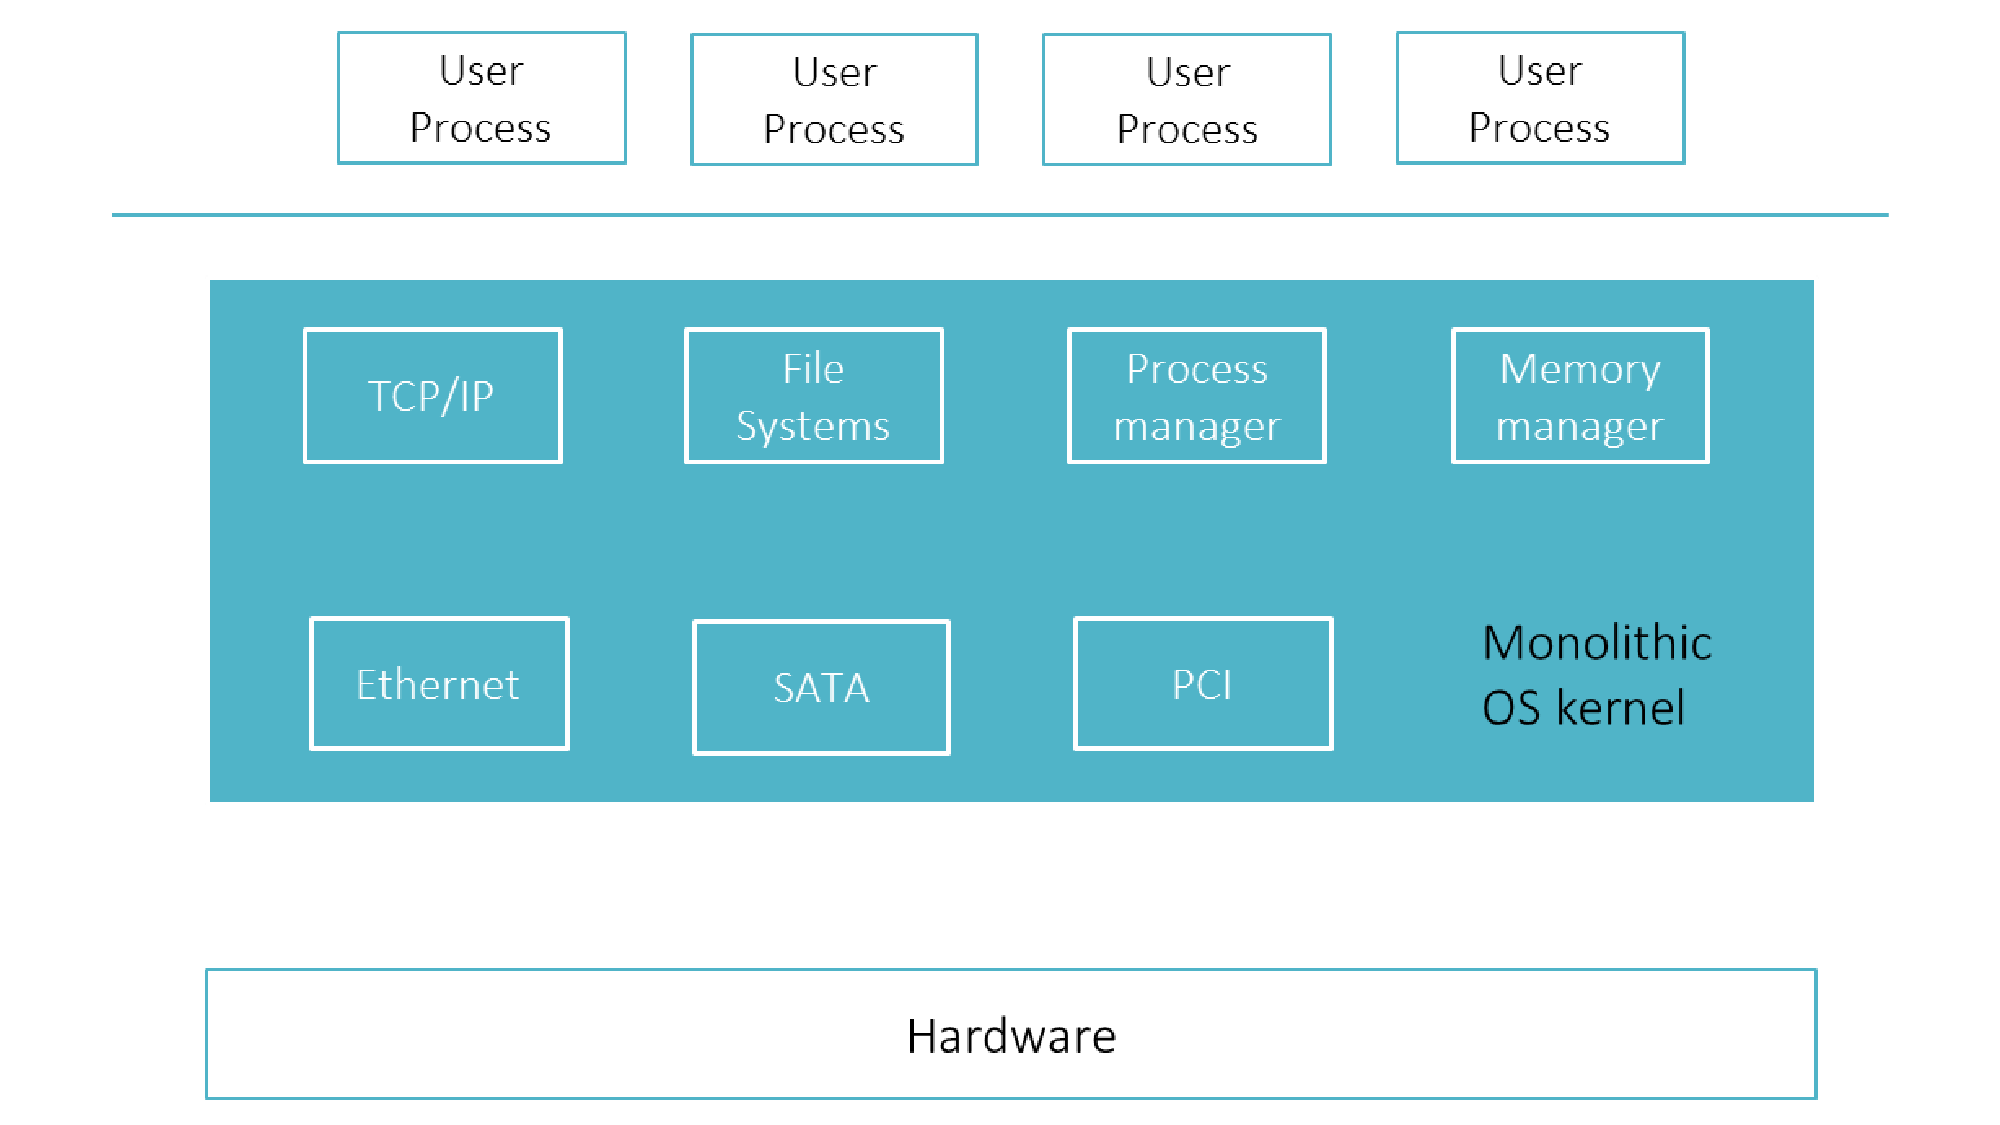
\includegraphics[scale=.5]{OSoverview}
\caption{Architectural overview of a modern OS}
\label{fig:monolithic}
\end{figure}

\begin{figure}[!ht]
\centering
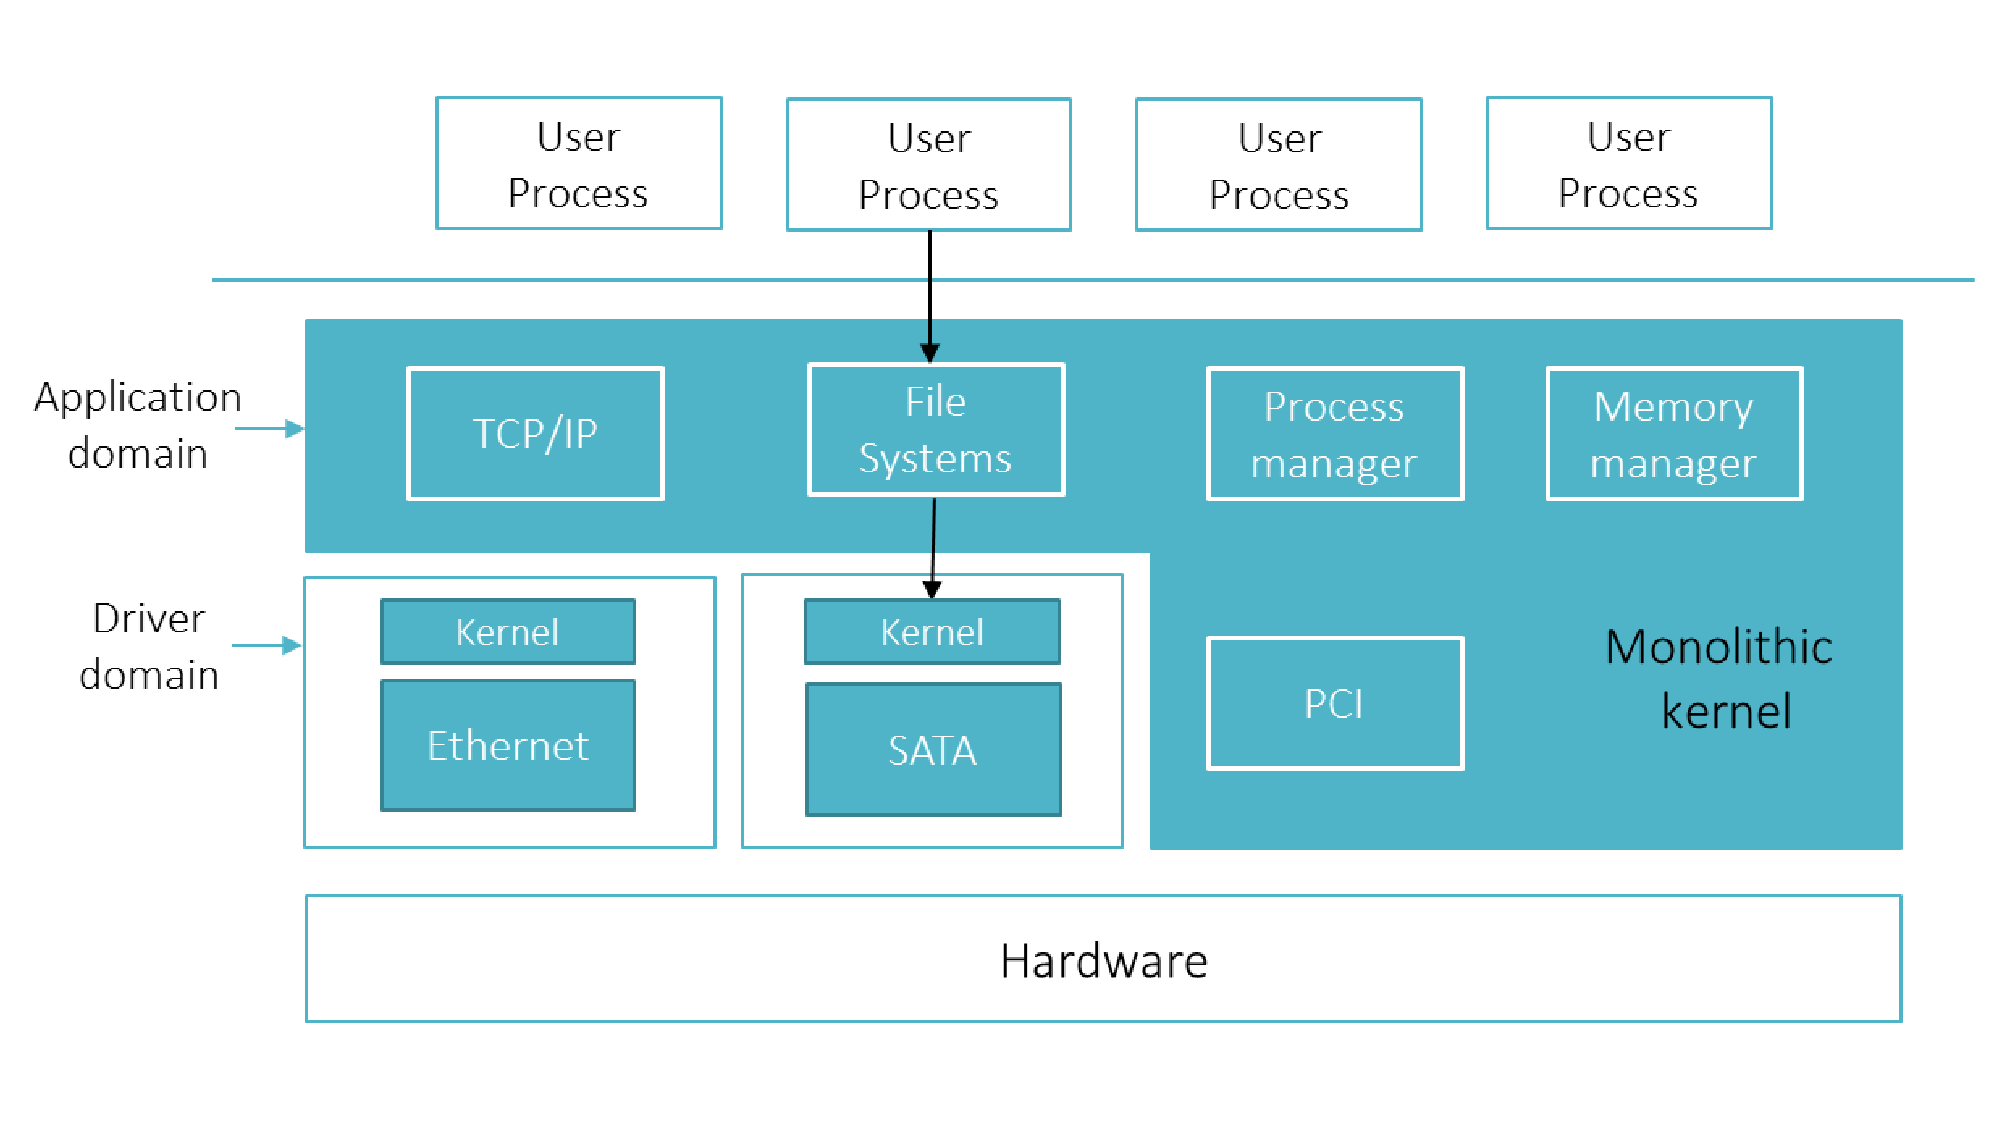
\includegraphics[scale=.5]{baseIDDRsystemoverview}
\caption{Architectural overview of the interrupt based IDDR system}
\label{fig:base IDDR system overview}
\end{figure}
The Figure~\ref{fig:base IDDR system overview} shows that IDDR system partitions an existing kernel into multiple independent components. User applications and the Linux kernel run in a domain called the \textit{application domain}. A device driver, which needs to be isolated from a kernel, executes in the separate domain called the \textit{driver domain}. Multiple domains run on the same hardware with the help of a VMM. User applications or kernel components access the hardware through the driver domain.
\\[3mm]
The goal of the IDDR system is to provide isolation between the device driver and the kernel. However, a device driver depends on kernel component such as a scheduler. Hence we run the device driver with an instance of a kernel and introduce a VMM into the design to run multiple kernels on a common hardware. 

\section{System Components}\label{components}
The section describes the 3 main components of the design - frontend driver, backend driver, and communication module.
\begin{figure}[!ht]
\centering
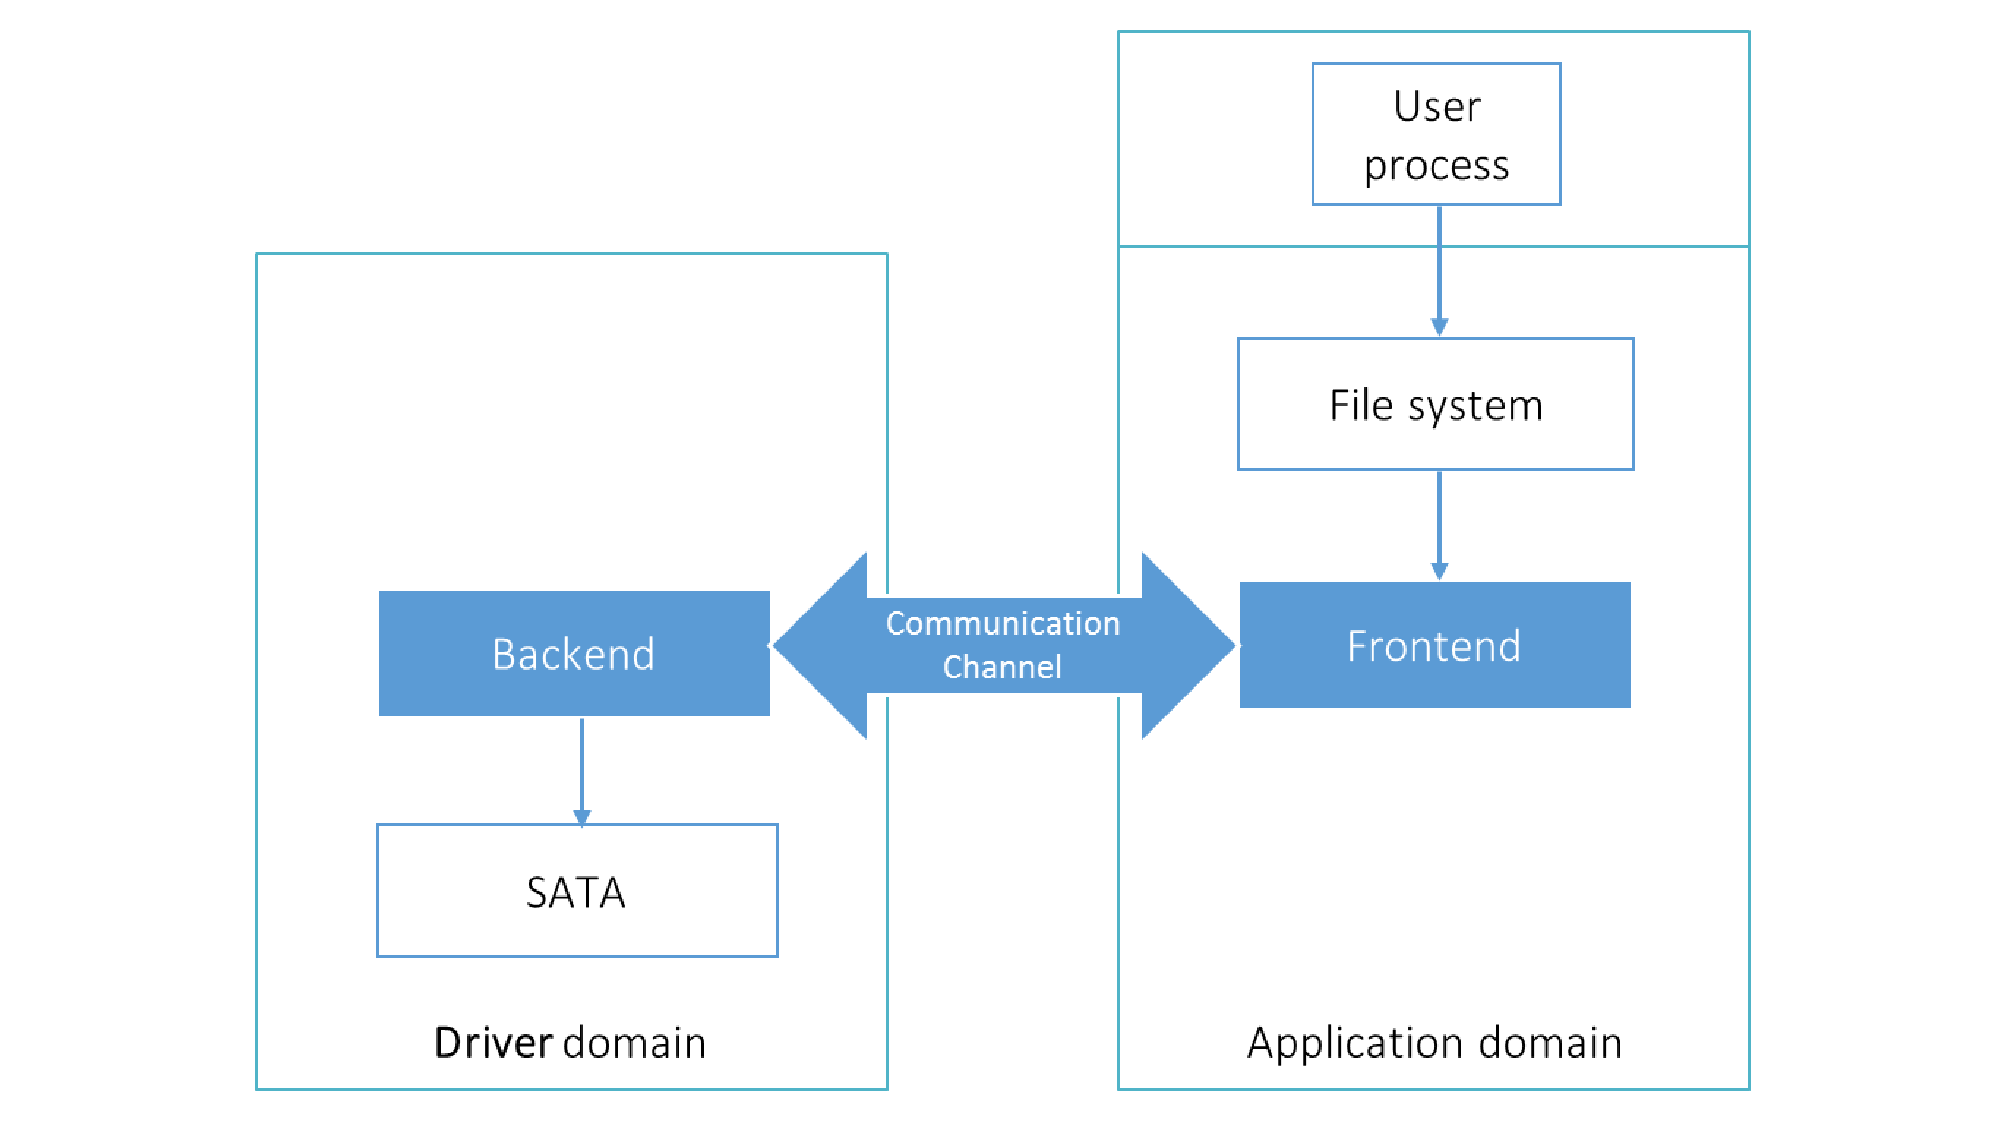
\includegraphics[scale=.5]{IDDRcomponents}
\caption{System Components}
\label{fig:Design Evo1}
\end{figure}

\subsection{Frontend Driver}
\label{subsec:frontend}
The IDDR system runs a piece of a code called the \textit{frontend driver} in an application domain. The \textit{frontend driver} acts as a substitute for the actual device driver. The main purpose of the \textit{frontend driver} is to accept requests from user applications, process the requests, enqueue the requests for the driver domain and notify the driver domain. The \textit{frontend driver} reads and processes the responses received from the driver domain and ends corresponding requests.

In a Linux system, user applications send requests to the actual device driver running in the same domain. However, in the IDDR system the actual device driver runs in a separate domain and the frontend driver helps user applications to forward requests to this actual device driver. Without the frontend device driver, we would have had to change existing applications in order to send requests to the actual device driver running in the driver domain. Hence, with introduction of the frontend driver we achieve the transperency goal.

\subsection{Backend Driver}
\label{subsec:backend}
The IDDR system runs a piece of a code called the \textit{backend driver} runs in the driver domain. The responsibility of the \textit{backend driver} is to accept requests from the application domain and forward them to the actual device driver. The \textit{backend driver} sends the responses and notifies the application domain after receiving the responses from the device driver.

In a Linux system, the actual device driver sends responses back to user applications running in the same domain. However, in the IDDR system, the backend driver sends responses to the frontend driver. Without the backend device driver, we would have had to change existing device drivers in order to send responses to user applications running in the application domain. Hence, with introduction of the backend driver we achieve the compatibility goal.

\begin{figure}[!ht]
    \centering
    \begin{subfigure}[b]{0.45\textwidth}
	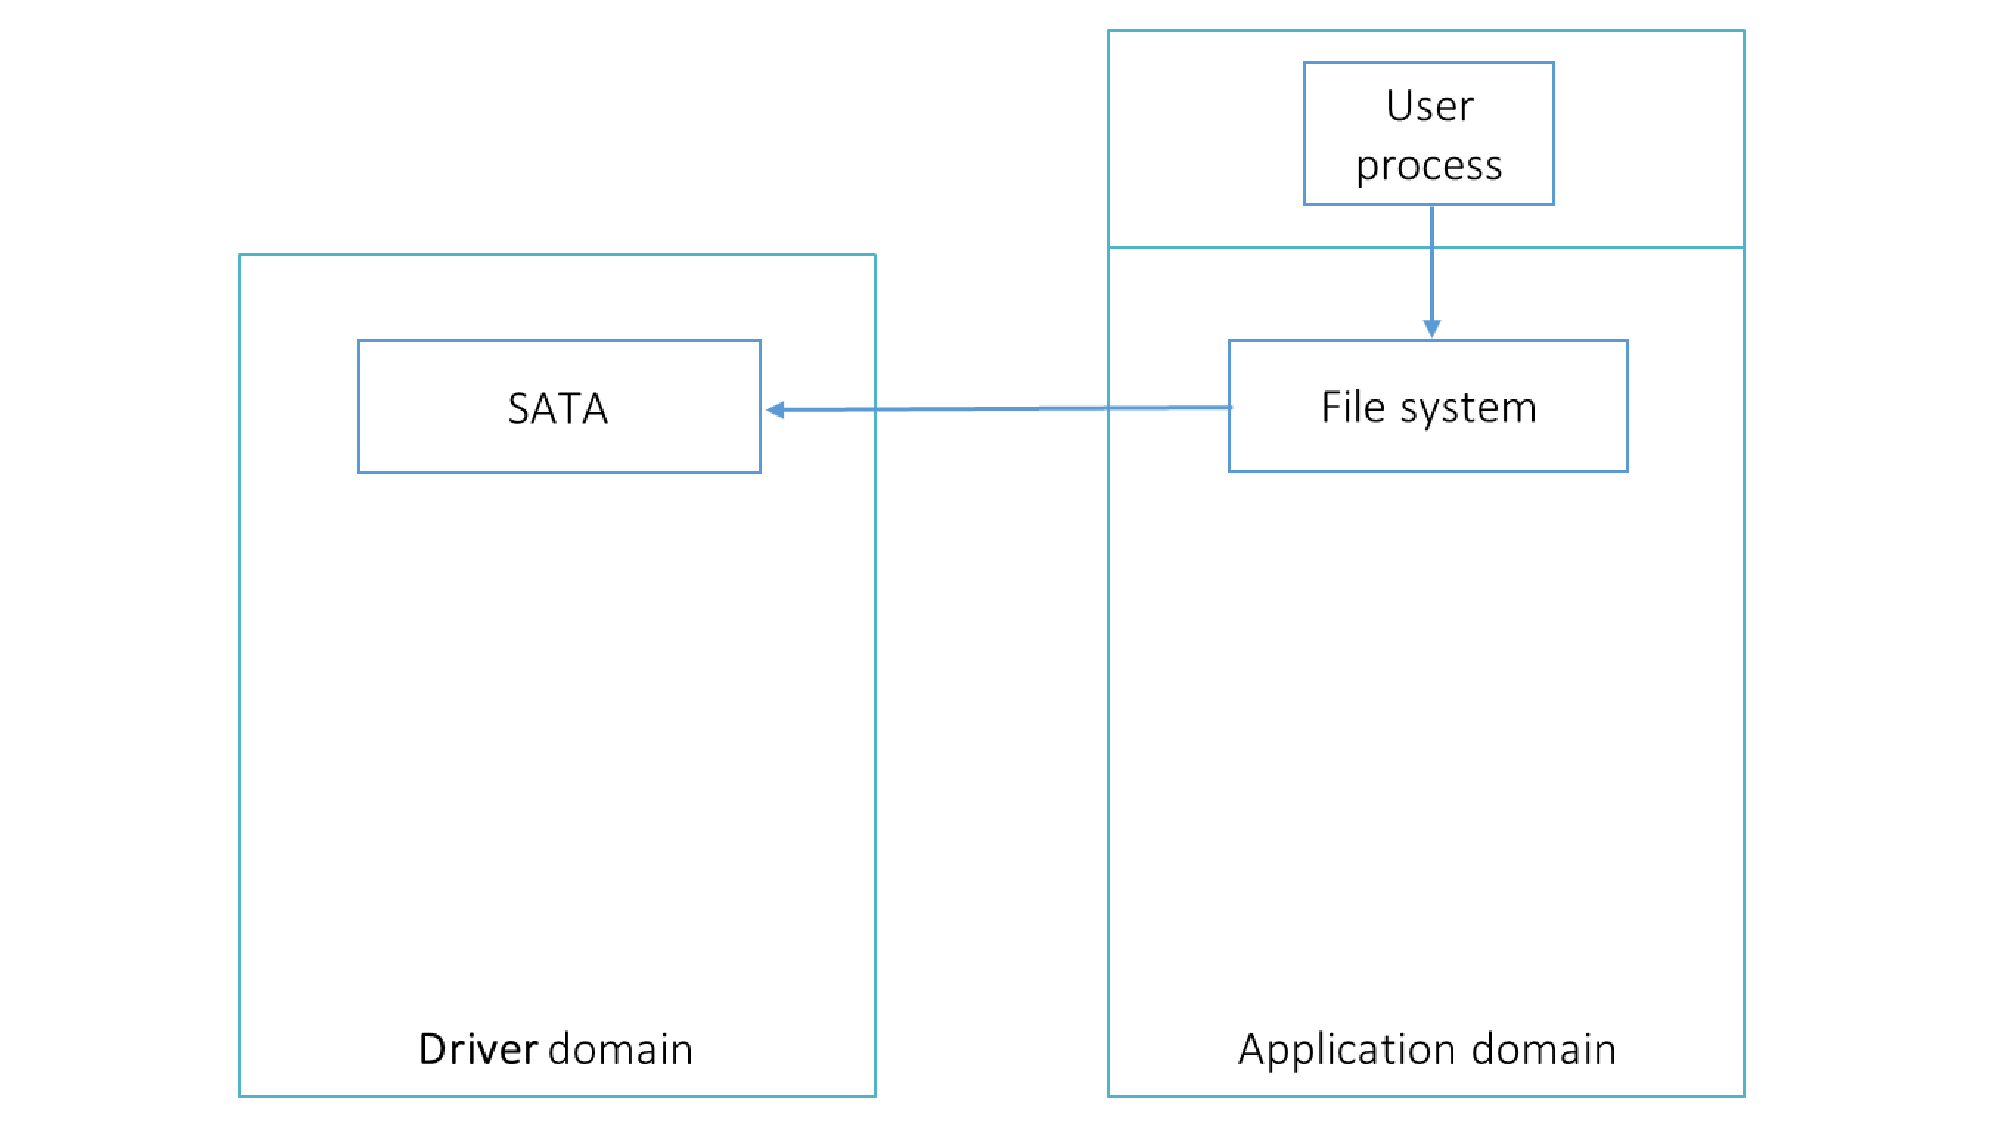
\includegraphics[scale=.25]{component1}
	\caption{Conceptual design of the driver domain}
	\label{fig:conept}
    \end{subfigure}
	\hfill
    \begin{subfigure}[b]{0.45\textwidth}
	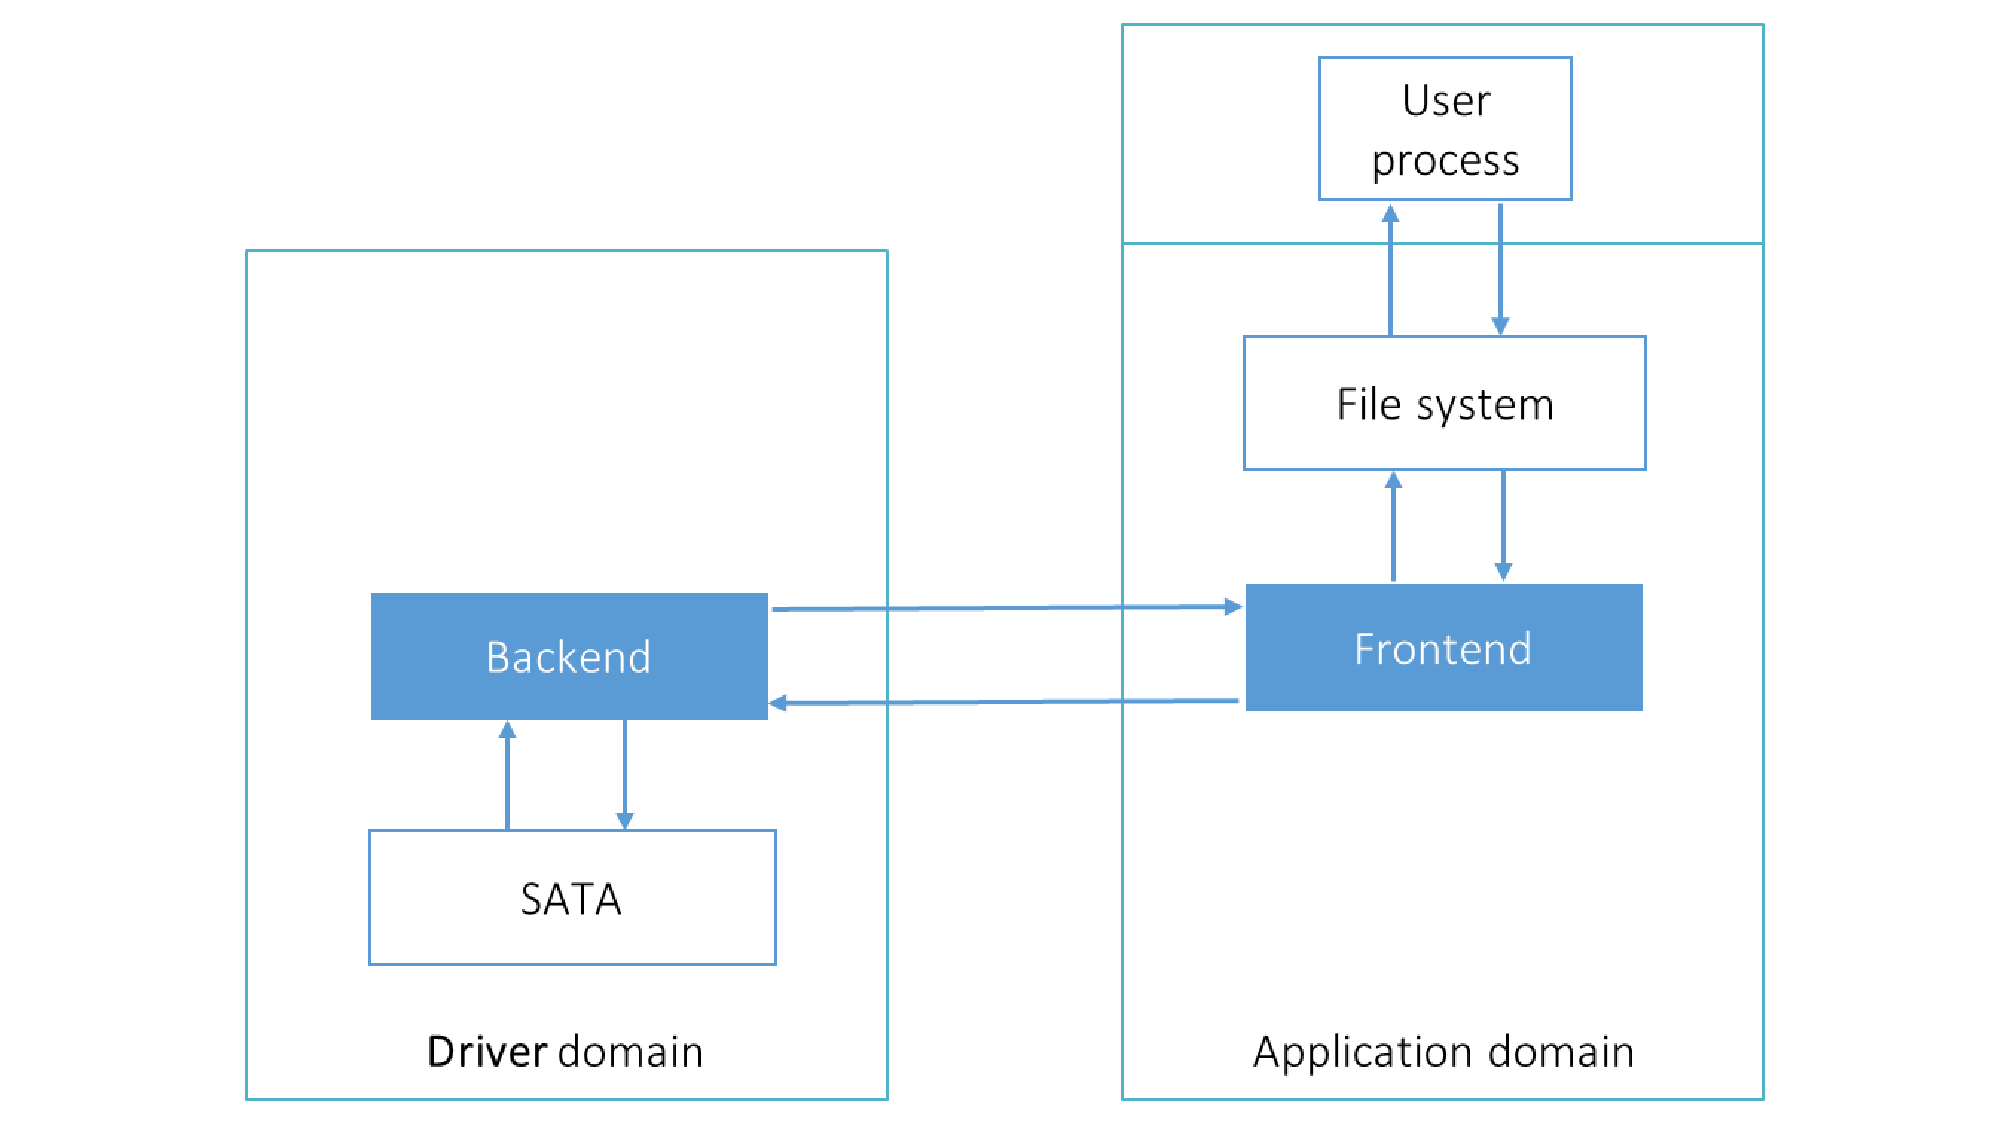
\includegraphics[scale=.25]{component2}
	\caption{Backend and frontend driver}
	\label{fig:backendfrontend}
    \end{subfigure}
    \caption{Role of the frontend and the backend drivers}\label{fig:fault tolerence}
\end{figure}

\subsection{Communication Module}
\label{sub:communicationmodule}
The communication module provides a communication channel between the \textit{frontend driver} and the \textit{backend driver}. The communication channel is logically divided into three parts. The responsibility of the communication module is to
\begin{enumerate} 
\item share the requests and responses between the driver domain and the application domain.
\item share the data of read/write requests/responses.
\item notify the domain upon the occurrence of a particular event. 
\end{enumerate}

Figure~\ref{fig:communication} provides the overview of the communication model. 
\begin{figure}[!ht]
\centering
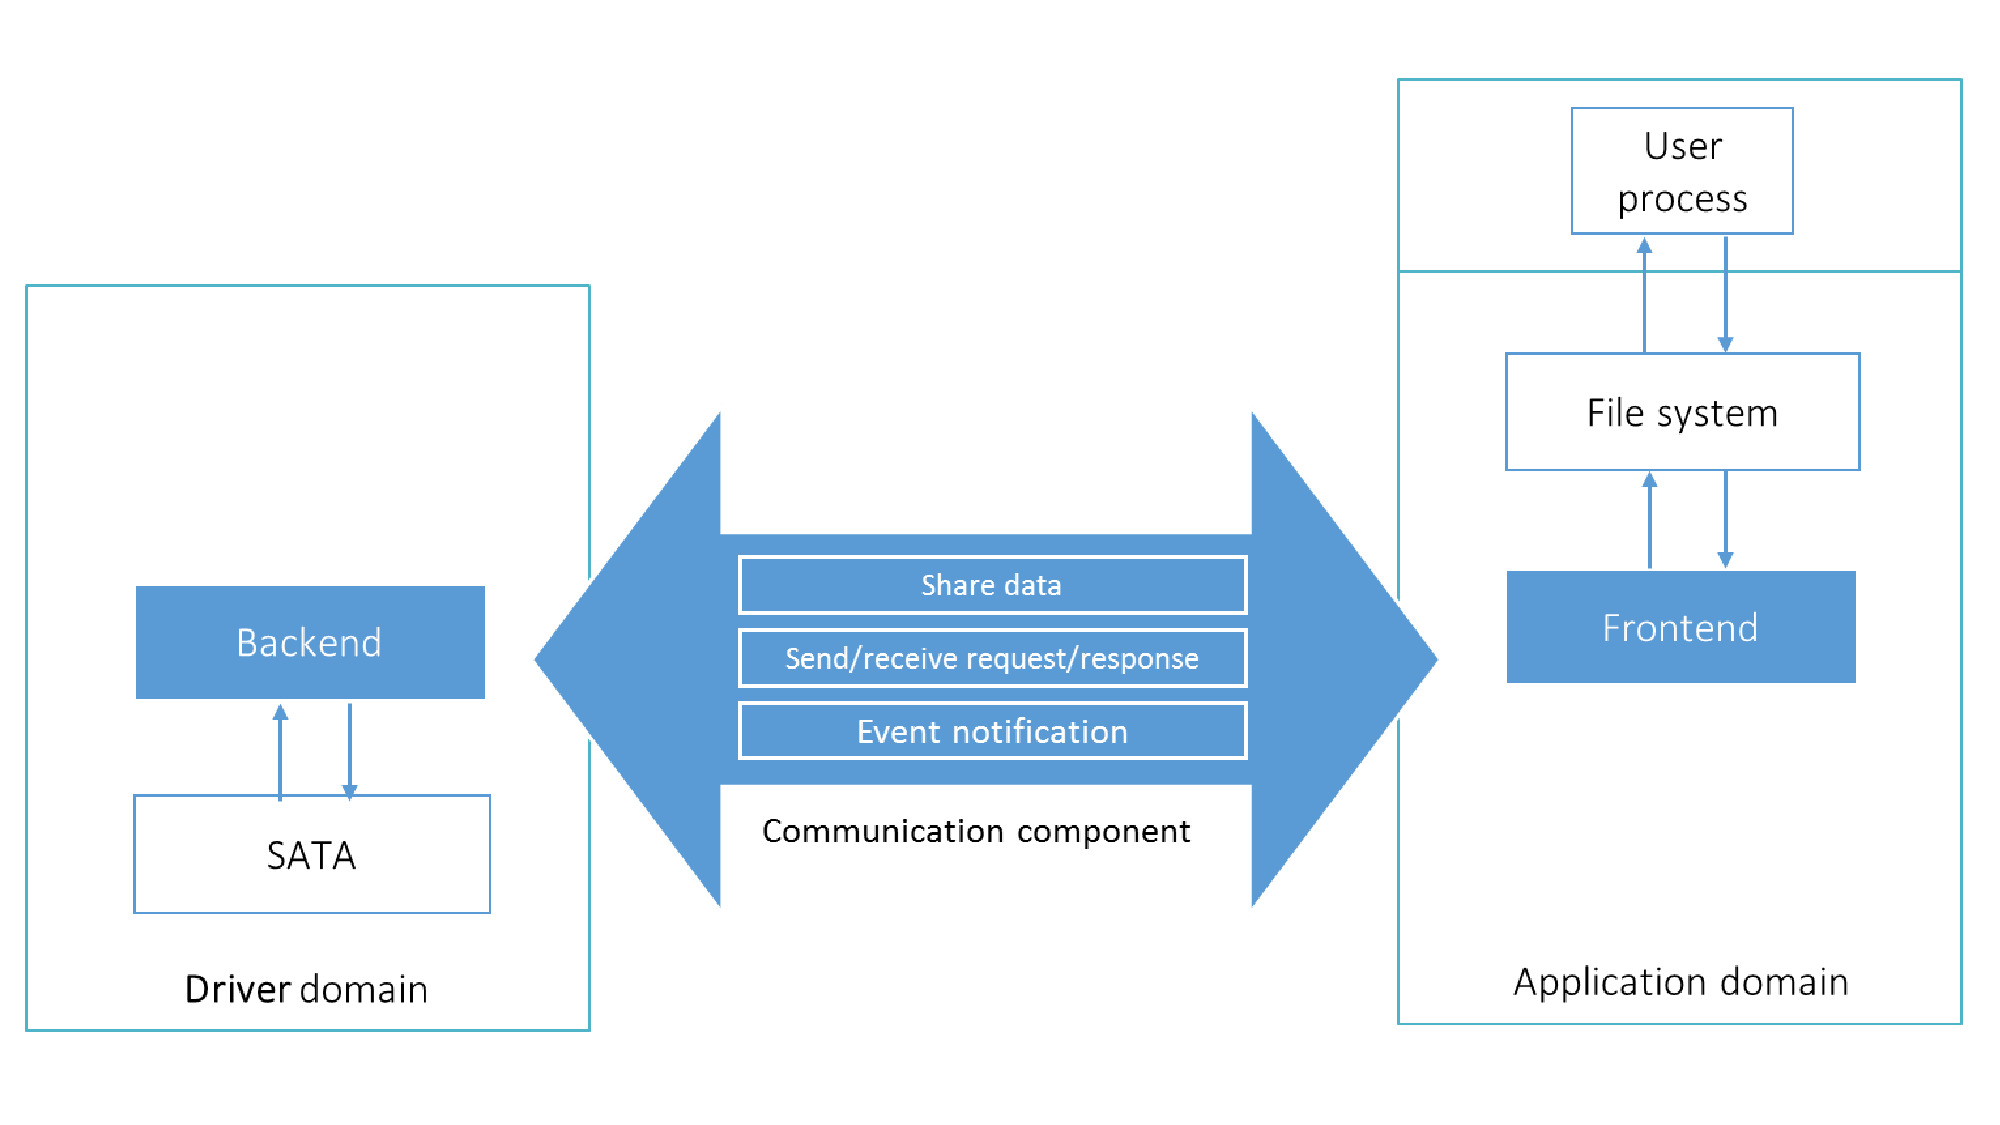
\includegraphics[scale=.5]{communicationmodule}
\caption{Communication Module}
\label{fig:communication}
\end{figure}

\section{System Design}\label{design}

The following section describes the design of interrupt based IDDR system and spinning based IDDR system. 

\subsection{Communication Module}

\paragraph{Interrupt based IDDR System:}
\label{par:base IDDR communication}
In interrupt based IDDR system, the frontend driver submits requests to the communication module. The communication module copies data of the write requests in a shared memory. The communication module is responsible for the allocation and de-allocation of the shared memory page. Once a sufficient number of requests is submitted by the frontend driver, the communication channel shares the requests with the backend driver. It notifies the backend driver that requests are available in a shared request queue.

\paragraph{Spinning Based IDDR System:}
\label{par:spin IDDR communication}
In the interrupt based IDDR system, by default a software interrupt is sent to the domain as a notification. Each such software interrupt causes the hypervisor to schedule the driver domain. Similarly, software interrupts which notify the availability of responses, causes the hypervisor to schedule the application domain. The scheduling of the driver domain and the application domain might result in a context switch. 

In order to avoid these context switches, we run an intermediate thread in the frontend driver and an intermediate thread in the backend driver. Both threads spin for the availability of requests and responses in the shared queue. The intermediate threads delegate the responsibility of the notifications from the frontend driver and backend driver to the communication module. 

\subsection{Frontend Driver}
\paragraph{Interrupt based IDDR System Design:}
In the IDDR system, the frontend driver provides an interface to accept requests from a user application on behalf of the device driver. As explained in Section~\ref{subsec:request queue}, each block device driver has a separate request queue to accept requests from a user application. Similar to block device drivers, the frontend driver also creates an individual request queue for a device to accept requests from user applications. The frontend driver flushes the requests to the communication channel. The frontend driver receives a software interrupt upon the availability of responses in the shared queue. The frontend driver handles the software interrupt by reading data from the shared memory in case of read operation and sends a completion notification to a user application. Otherwise it sends a completion notification to a user application.

\paragraph{IDDR System Design:}
As explained in Section~\ref{par:spin IDDR communication}, we introduce an intermediate thread to read responses from the shared queue. The intermediate thread spins for responses. Upon availability of a response, the thread reads the response and sends a complition notification to a user application. If the corresponding request is a read request, then the thread reads the shared data too.

\begin{figure}[!ht]
\centering
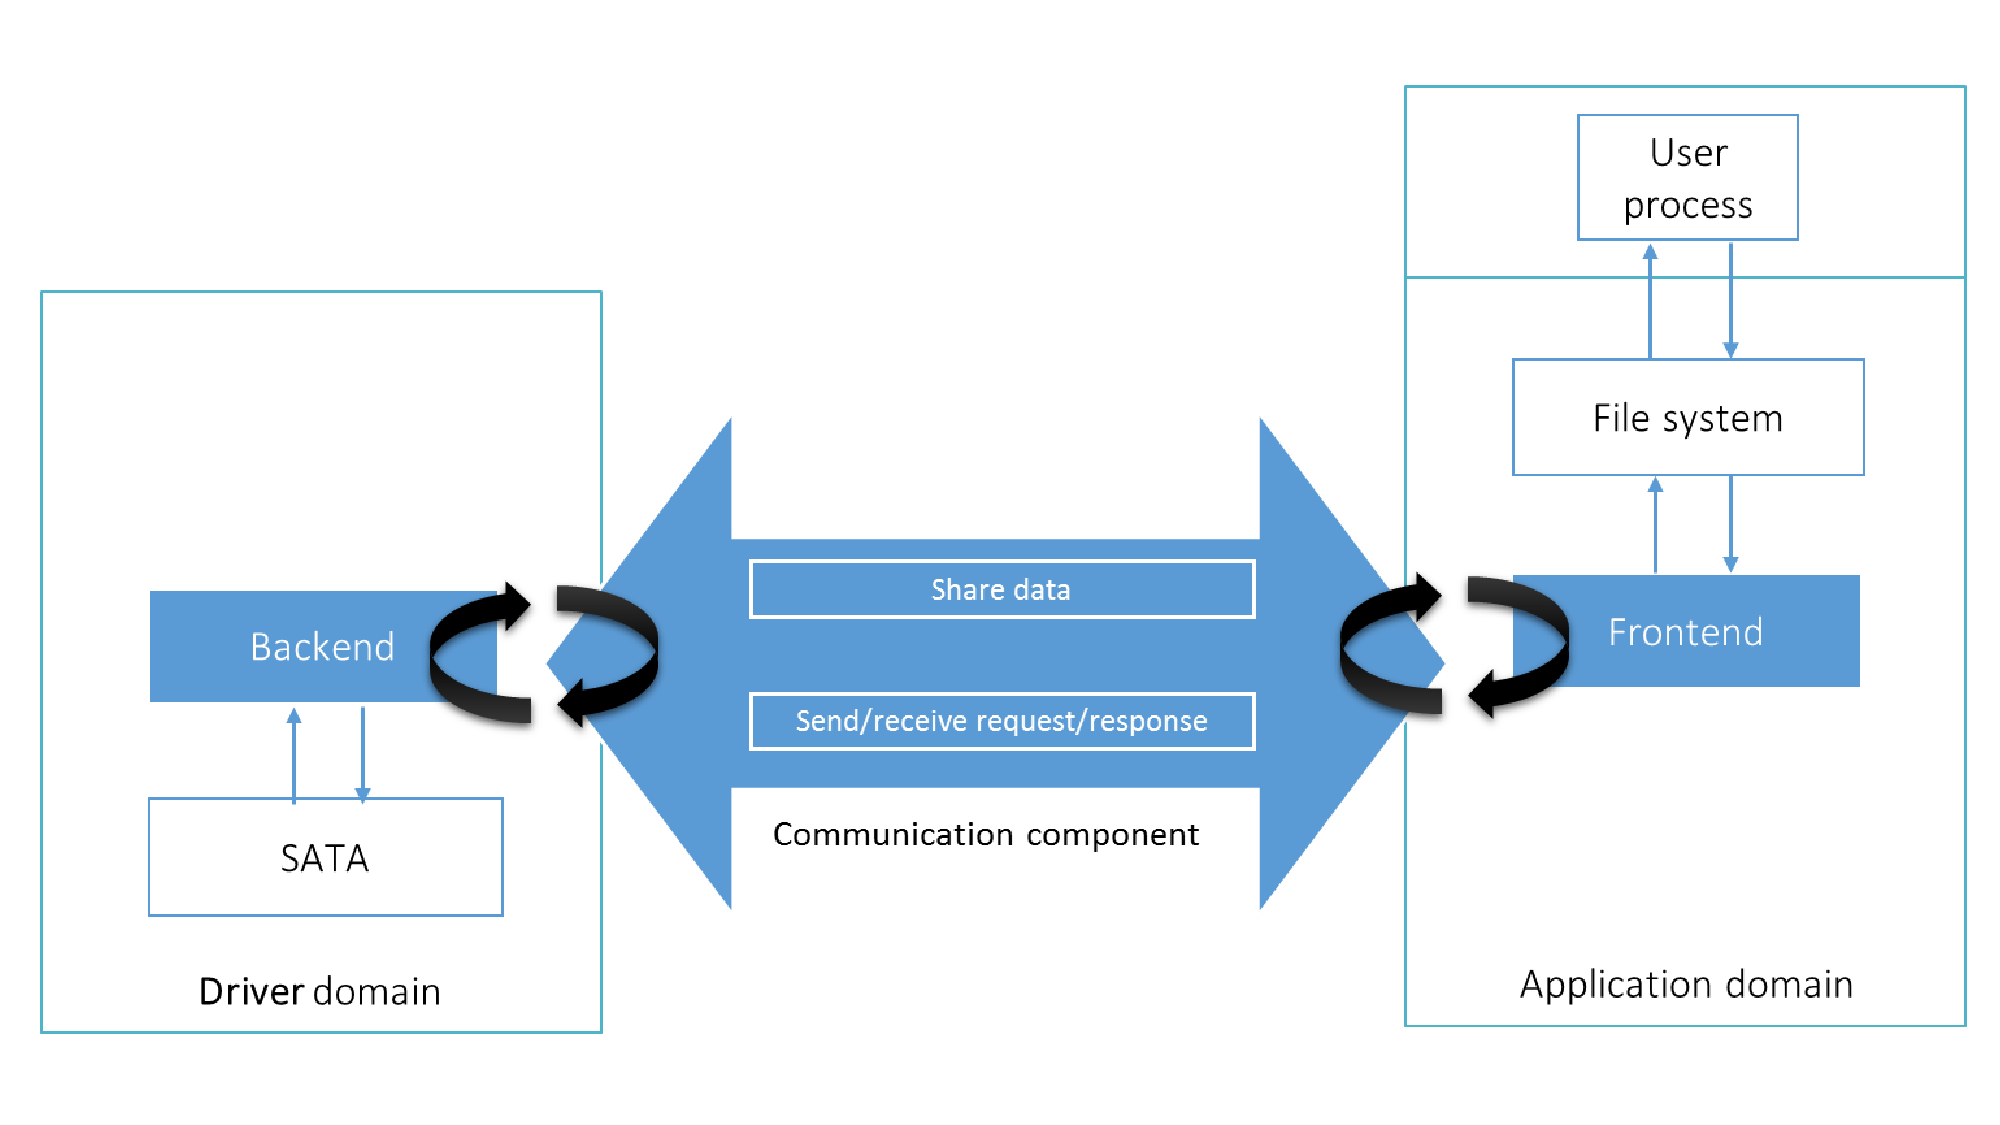
\includegraphics[scale=.5]{IDDRdesign}
\caption{Spinning based IDDR system}
\label{fig:new IDDR system}
\end{figure}

% \section{fault tolerance}
% Figure~\ref{fig:driver crash} and Figure~\ref{fig:high avail} explains the effects of a malicious activity occurring in the device driver isolated from the Linux kernel. When a device driver running in a driver domain hits a bug, it crashes the kernel of the driver domain and hence the driver domain itself. In addition, applications expecting a response from the driver domain might hang or crash waiting for the response. But due to the address space separation of the application domain and the driver domain, the application domain will remain intact.   
% \begin{figure}[!ht]
%     \centering
%     \begin{subfigure}[b]{0.45\textwidth}
% 	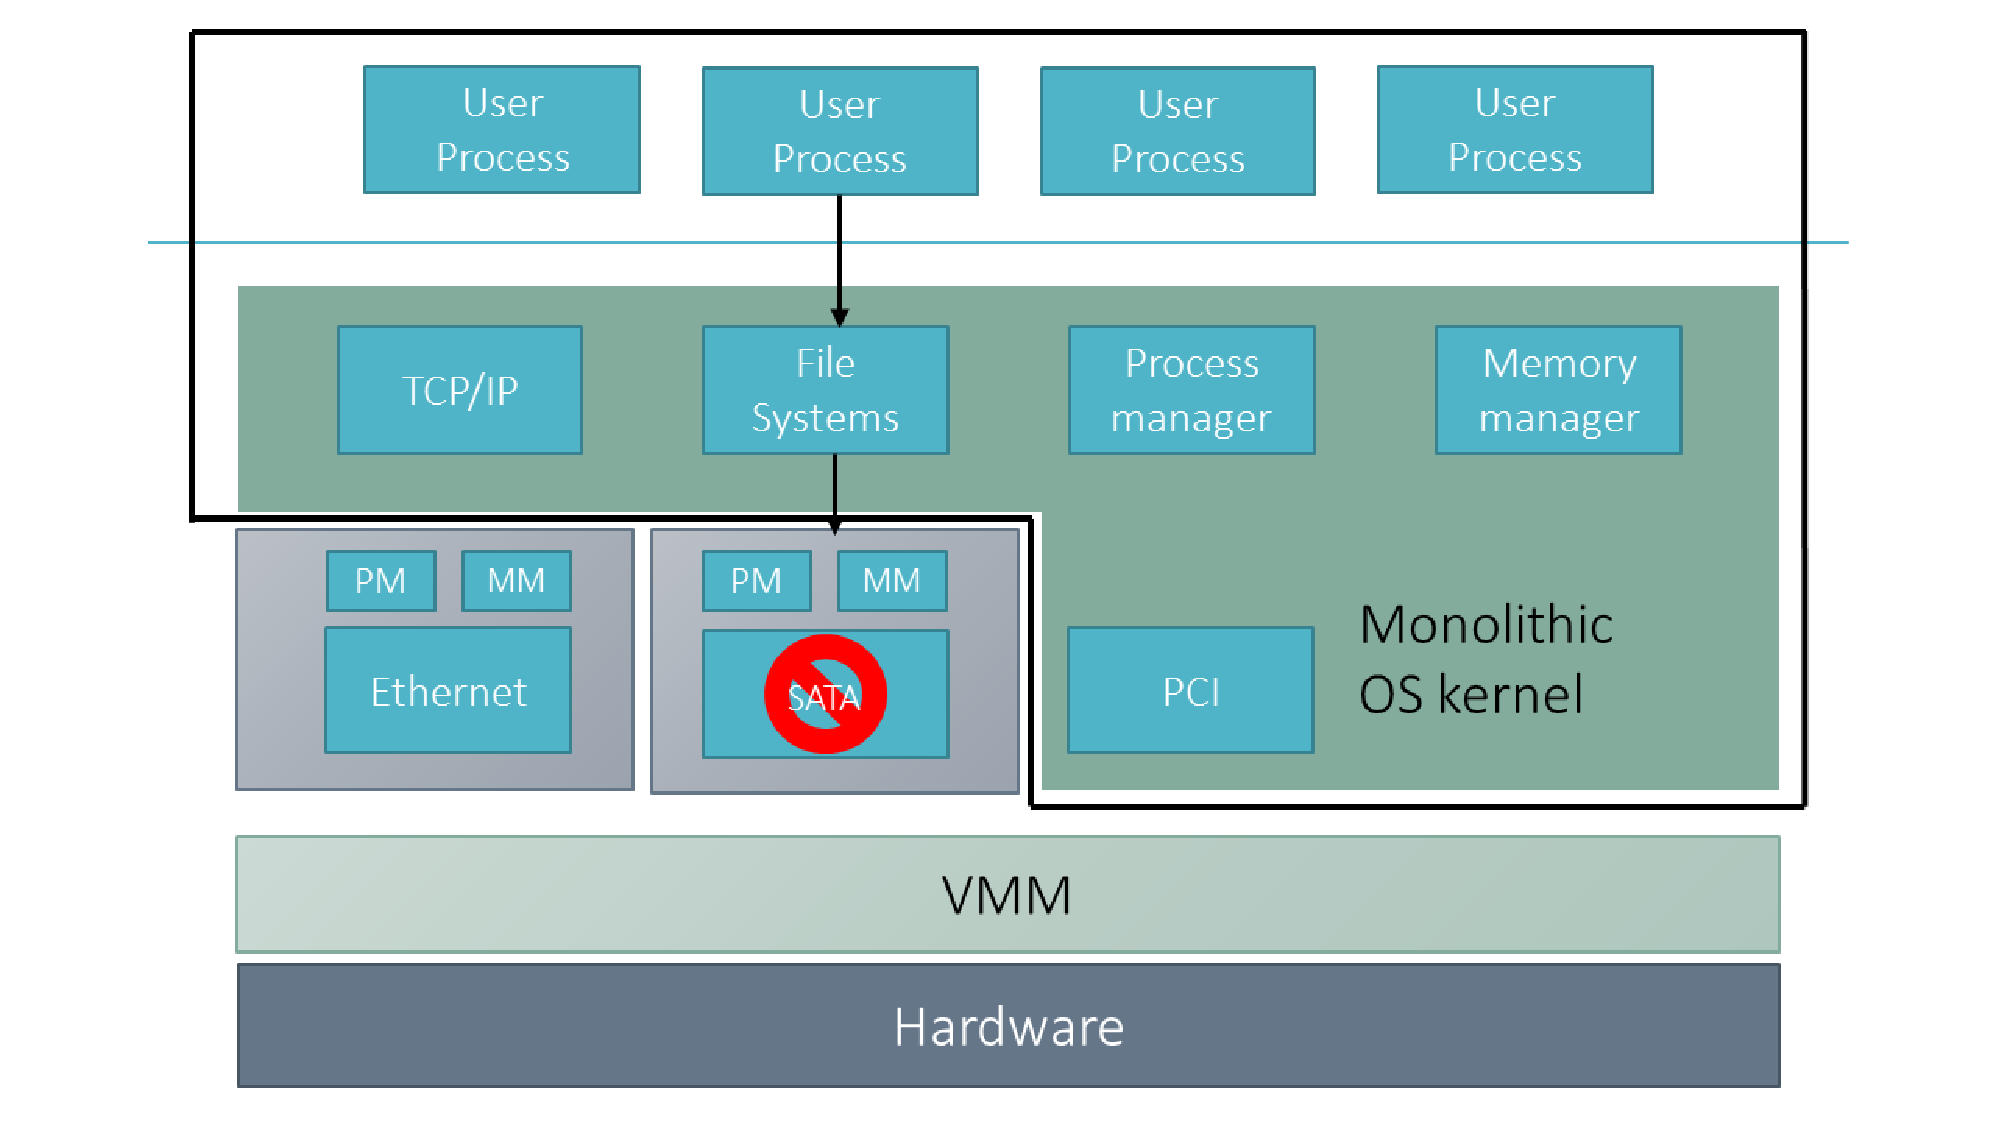
\includegraphics[scale=.25]{IDDRcrash1}
% 	\caption{Device driver crash}
% 	\label{fig:driver crash}
%     \end{subfigure}
% 	\hfill
%     \begin{subfigure}[b]{0.45\textwidth}
% 	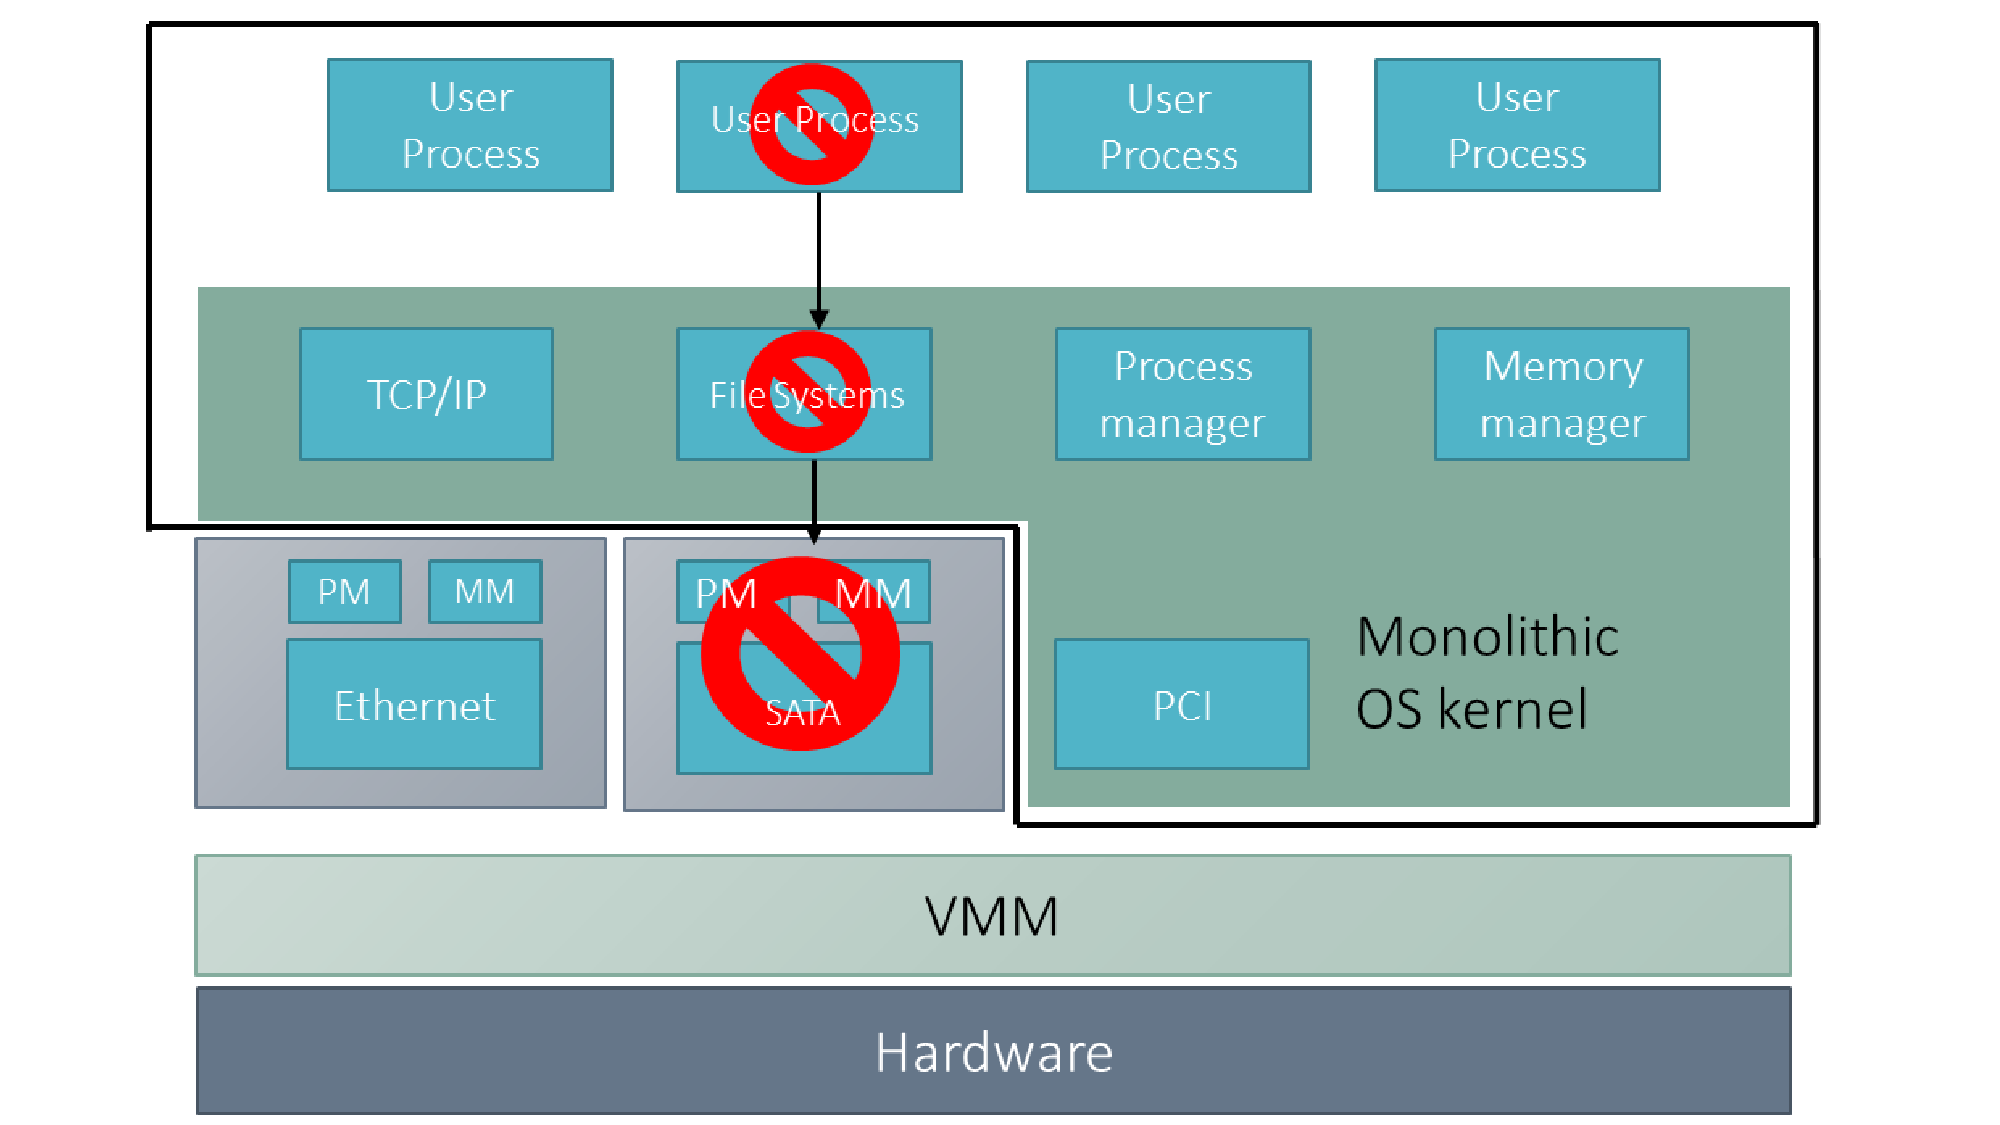
\includegraphics[scale=.25]{IDDRcrash2}
% 	\caption{Intact system}
% 	\label{fig:high avail}
%     \end{subfigure}
%     \caption{Fault tolerence}\label{fig:fault tolerence}
% \end{figure}
    
\ifbool{toShowBibliography}{\bibliography{references}}{}
